\documentclass{beamer}
\usepackage{amsmath}
\usepackage{amssymb}
\usepackage{booktabs}
\usepackage{rotating}
\usepackage{multirow}
\usepackage{colortbl,color}
\usepackage{graphics}
\usetheme{default}
\renewcommand{\theenumii}{\alph{\enumii}}
\defbeamertemplate{itemize subitem}{dash}{--}
\defbeamertemplate{itemize subsubitem}{dash}{--}
\setbeamertemplate{itemize item}[circle]
\setbeamertemplate{itemize subitem}[dash]
\setbeamertemplate{itemize subsubitem}[dash]
\setbeamertemplate{enumerate item}{\arabic{enumi}.}
\setbeamertemplate{enumerate subitem}{(\alph{enumii})}
\usefoottemplate{}
\newcommand{\RedOverlay}[1]{\only{\color{red}{#1} }}
\newcommand{\UNCOVER}[3]{\only<#2>{\color{white}{#1}}\only<#3>{#1}}
\newcommand{\UNCOVERR}[4]{\only<#2>{\color{white}{#1}}\only<#3>{\color{red}{#1}}\only<#4>{#1}}
\newcommand{\showOn}[3]{\only<#2>{\color<#2>{black} #1}\only<#3>{\color<#3>{white} #1}}
\setbeamertemplate{headline}{}
\usenavigationsymbolstemplate{}
\setbeamercolor{titlelike}{fg=black}
\setbeamercolor{item}{fg=black}

\newcommand{\indicator}[1]{\mathrm{1}\left\{{#1}\right\}}



\begin{document}

\title{\LARGE Communication in Multiple Dimensions with Multiple Experts}
\author{\begin{tabular}{cc}
	Emanuel I. Vespa & Alistair J. Wilson
	\\ {\tiny{UCSB}} & {\tiny{Pitt}} \\
\end{tabular} }
\date{Stanford, 2016}
\maketitle
\begin{frame}{Research Question:}

{\Large
	Can competition between biased information sources lead to more informed consumers?
 }
\end{frame}

\begin{frame}{Theory Summary}
	\begin{itemize}
		\item With just one sender and misaligned preferences, there is no full-revelation
		\item Additional senders in one dimension leads to possibility of more information transfer, but not robust
		\item With multiple dimensions, competition between senders generically leads to existence of fully revealing equilibrium.
	\end{itemize}
\end{frame}


\subsection{Theory}
\begin{frame}{Theory}
	\begin{center}
		\begin{tabular}{ccc} \toprule
		Policy Dimension	&  One-Sender   & Multiple-Senders   \\  \midrule
		Univariate			&  \showOn{Crawford \& Sobel}{2}{1} &   \color{white}{Krishna \& Morgan} \\
		Multivariate		&	\color{white}{Crawford \& Sobel} &	\color{white}{Battaglini}	\\  \bottomrule
		\end{tabular}
	\end{center}
\end{frame}

\begin{frame}{Theory}
	\begin{center}
		\begin{tabular}{ccc} \toprule
		Policy Dimension	&  One-Sender   & Multiple-Senders   \\  \midrule
		Univariate			&  Crawford \& Sobel &   \showOn{Krishna \& Morgan}{2}{1} \\
		Multivariate		& \color{white}{Crawford \& Sobel}  &	\color{white}{Battaglini} \\  \bottomrule
		\end{tabular}
	\end{center}
\end{frame}

\begin{frame}{Krishna-Morgan, Misaligned Senders}
	\begin{center}
		\includegraphics<1>[width=1.0\textwidth]{../../../../ARCHIVE/vw_multi2/Images/GJexample-1.eps}
		\includegraphics<2>[width=1.0\textwidth]{../../../../ARCHIVE/vw_multi2/Images/GJexample-2.eps}
		\includegraphics<3>[width=1.0\textwidth]{../../../../ARCHIVE/vw_multi2/Images/GJexample-3.eps}
		\includegraphics<4>[width=1.0\textwidth]{../../../../ARCHIVE/vw_multi2/Images/GJexample-4.eps}
		\includegraphics<5>[width=1.0\textwidth]{../../../../ARCHIVE/vw_multi2/Images/GJexample-5.eps}
		\includegraphics<6->[width=1.0\textwidth]{../../../../ARCHIVE/vw_multi2/Images/GJexample-6.eps}
	\end{center}
	\only<1>{State realized}
	\only<2>{Two advisers either side of you}
	\only<3>{Two messages, one from each adviser}
	\only<4>{Equilibrium: if they agree, choose their recommendation}
	\only<5-6>{Equilibrium: if they disagree, punish}
	\only<7>{Non-robust: small errors? non-credible threat?}

\end{frame}


\begin{frame}{Theory}
	\begin{center}
		\begin{tabular}{ccc} \toprule
		Policy Dimension	&  One-Sender   & Multiple-Senders   \\  \midrule
		Univariate			&  Crawford \& Sobel &   Krishna \& Morgan \\
		Multivariate		& \showOn{Crawford \& Sobel}{2}{1} &	\color{white}{Battaglini}	\\  \bottomrule
		\end{tabular}
	\end{center}
\end{frame}
\begin{frame}{Multidimensional Example}
	\begin{center}
		\includegraphics<1>[width=0.7\textwidth]{../../../../ARCHIVE/vw_multi2/Images/SenderPrefs0-1.eps}
		\includegraphics<2>[width=0.7\textwidth]{../../../../ARCHIVE/vw_multi2/Images/SenderPrefs0-2.eps}
		\includegraphics<3>[width=0.7\textwidth]{../../../../ARCHIVE/vw_multi2/Images/SenderPrefs0-2-5.eps}
		\includegraphics<4>[width=0.7\textwidth]{../../../../ARCHIVE/vw_multi2/Images/SenderPrefs0-3.eps}
		\includegraphics<5>[width=0.7\textwidth]{../../../../ARCHIVE/vw_multi2/Images/SenderPrefs0-4.eps}
		\includegraphics<6>[width=0.7\textwidth]{../../../../ARCHIVE/vw_multi2/Images/SenderPrefs0-5.eps}
	\end{center}
\end{frame}


\begin{frame}{Theory}
	\begin{center}
		\begin{tabular}{ccc} \toprule
		Policy Dimension	&  One-Sender   & Multiple-Senders   \\  \midrule
		Univariate			&  Crawford \& Sobel &   Krishna \& Morgan \\
		Multivariate		&  Crawford \& Sobel &	\showOn{Battaglini}{2}{1}	\\  \bottomrule
		\end{tabular}
	\end{center}
\end{frame}

\begin{frame}{Multidimensional, Multi-Sender Example}
	\begin{center}
		\includegraphics<1>[width=0.8\textwidth]{../../../../ARCHIVE/vw_multi2/Images/SenderPrefs0.eps}
		\includegraphics<2>[width=0.8\textwidth]{../../../../ARCHIVE/vw_multi2/Images/SenderPrefs3-1.eps}
		\includegraphics<3>[width=0.8\textwidth]{../../../../ARCHIVE/vw_multi2/Images/SenderPrefs3-2.eps}
		\includegraphics<4>[width=0.8\textwidth]{../../../../ARCHIVE/vw_multi2/Images/SenderPrefs3-3.eps}
		\includegraphics<5>[width=0.8\textwidth]{../../../../ARCHIVE/vw_multi2/Images/SenderPrefs3-4.eps}
		\includegraphics<6>[width=0.8\textwidth]{../../../../ARCHIVE/vw_multi2/Images/SenderPrefs3-2.eps}
		\includegraphics<7>[width=0.8\textwidth]{../../../../ARCHIVE/vw_multi2/Images/ReceiverPrefs1.eps}
		\includegraphics<8>[width=0.8\textwidth]{../../../../ARCHIVE/vw_multi2/Images/ReceiverPrefs2.eps}
		\includegraphics<9>[width=0.8\textwidth]{../../../../ARCHIVE/vw_multi2/Images/Equilib1-3.eps}
		\includegraphics<10>[width=0.8\textwidth]{../../../../ARCHIVE/vw_multi2/Images/Equilib1-1.eps}
		\includegraphics<11>[width=0.8\textwidth]{../../../../ARCHIVE/vw_multi2/Images/Equilib1-2.eps}
		\includegraphics<12>[width=0.8\textwidth]{../../../../ARCHIVE/vw_multi2/Images/Equilib1-3.eps}
		\includegraphics<13>[width=0.8\textwidth]{../../../../ARCHIVE/vw_multi2/Images/Equilib2-3.eps}
		\includegraphics<14>[width=0.8\textwidth]{../../../../ARCHIVE/vw_multi2/Images/Equilib2-1.eps}
		\includegraphics<15>[width=0.8\textwidth]{../../../../ARCHIVE/vw_multi2/Images/Equilib2-2.eps}
		\includegraphics<16>[width=0.8\textwidth]{../../../../ARCHIVE/vw_multi2/Images/Equilib2-3.eps}
	\end{center}
\end{frame}
\begin{frame}{Alternative Solution}
	\begin{itemize}
		\item Suppose the players exaggerate in the direction of their bias:
		$$\mathbf{x}(\boldsymbol{\theta})=\boldsymbol{\theta}+k_x \cdot \boldsymbol{\delta}_X $$
		$$\mathbf{y}(\boldsymbol{\theta})=\boldsymbol{\theta}+k_y \cdot \boldsymbol{\delta}_Y $$
		where $k_X$ and $k_Y$ represent the degree of exaggeration.\pause
		\item Eliminating the unknown state $\boldsymbol{\theta}$ we get:
		$$\mathbf{y}(\boldsymbol{\theta})-\mathbf{x}(\boldsymbol{\theta})=k_Y \cdot \boldsymbol{\delta}_Y-k_X \cdot \boldsymbol{\delta}_X$$ \pause
		\item But only $k_X$ and $k_Y$ are unknowns---2 unknowns in $n\geq2$ equations.\pause
		%\item So the receiver makes a choice:
		%		$$\mathbf{x}-k_x\left(\mathbf{y}-\mathbf{x};\boldsymbol{\delta}_X,\boldsymbol{\delta}_Y\right)\cdot\boldsymbol{\delta}_X $$
		%

	\end{itemize}
\end{frame}
\begin{frame}{Alternative Solution Example}
	\begin{itemize}
		\item Consider the case where:
		$$\boldsymbol{\delta}_X=\left( \begin{array}{c} -1 \\ 1 \end{array} \right)\text{ and } \boldsymbol{\delta}_Y=\left( \begin{array}{c} 1 \\ 1\end{array}\right)$$\pause
		\item We therefore know that:
		$$\left(\begin{array}{r} y_1-x_1 \\ y_2-x_2 \end{array}\right) =\left(\begin{array}{r} k_y+k_x \\ k_y-k_x \end{array}\right)$$\pause
		\item So the difference in the two recommendations tells us
		\begin{enumerate}
			\item The sum of their exaggerations
			\item The difference in the exaggerations.
		\end{enumerate}
	\end{itemize}
\end{frame}
\begin{frame}{Theory}
	\begin{center}
		\begin{tabular}{ccc} \toprule
		Policy Dimension	&  One-Sender   & Multiple-Senders   \\  \midrule
		Univariate			& No Full Revelation &   Non-Robust Equilibria \\
		Multivariate		&  No Full Revelation &	Full Revelation	\\  \bottomrule
		\end{tabular}
	\end{center}
\end{frame}

\subsection{Experiment}
\begin{frame}{How do we implement this in the lab?}
	\begin{itemize}
		\item Two dimensions.
		\item 3 subjects in a group:
		\begin{itemize}
			\item 2 Senders with differing biases
			\begin{itemize}
				\item Each sends a message in the plane
			\end{itemize}
			\item 1 Receiver
			\begin{itemize}
				\item Given the two messages, chooses a point in the plane.
			\end{itemize}
		\end{itemize}
		\item Pay the subjects \$20 if chosen point is their best location
		\item Payoffs decreasing in the distance from chosen point
	\end{itemize}
\end{frame}

\begin{frame}{Problems with boundedness}
	\includegraphics<1>[width=0.8\textwidth]{../../../../ARCHIVE/vw_multi2/Images/Bounded1.eps}
	\includegraphics<2>[width=0.8\textwidth]{../../../../ARCHIVE/vw_multi2/Images/Bounded.eps}
	\includegraphics<3>[width=0.8\textwidth]{../../../../ARCHIVE/vw_multi2/Images/Bounded2.eps}
\end{frame}

\begin{frame}{Solution to boundedness}
	\begin{itemize}
		\item We use two clocks as the state space, one for each dimension
		\item We relocate the Euclidean plane to the surface of a ``clifford torus''
			\begin{itemize}
				\item No boundaries to consider
				\item Can use a non-modal uniform distribution
			\end{itemize}
	\end{itemize}
\end{frame}

\begin{frame}{General Design}
	\begin{itemize}
		\item Between subject
		\begin{itemize}
			\item Treatment consist of an orientation
			% \item Randomize axes and sender identities
		\end{itemize}
		\item Fifteen rounds with role switching every 5: $X$, $Y$ and $Z$
		\item Last five rounds everyone is the receiver $Z$
		\begin{itemize}
			\item Generate extra data for receivers
			\item Remove other-regarding concerns
		\end{itemize}
	\end{itemize}
\end{frame}

\begin{frame}{Preferences}
	\begin{itemize}
		\item Every subject in the game is told their best point
			\begin{itemize}
				\item Receiver is the true state
				\item Senders are the true state plus their bias
			\end{itemize}
		\item Monetary payoffs are given by:
		$$\min\left\{ \$5,\$20-\$8\frac{\sqrt{\textrm{(\small Distance Best \ensuremath{1})}^{2}+\textrm{(\small Distance Best \ensuremath{2})}^{2}}}{45^{\circ}}\right\}$$
		\item Final payment is two random rounds.
	\end{itemize}
\end{frame}

\begin{frame}{Treatment\only<1>{---Axis Aligned}\only<2>{---Symmetric Rotated}}
	\includegraphics<1>[width=0.8\textwidth]{../../../../ARCHIVE/vw_multi2/Images/TreatmentAA.eps}
	\includegraphics<2>[width=0.8\textwidth]{../../../../ARCHIVE/vw_multi2/Images/TreatmentSR.eps}
	% \includegraphics<2>[width=0.8\textwidth]{../../../../ARCHIVE/vw_multi2/Images/TreatmentAR.eps}
\end{frame}

\begin{frame}{Round Details}
	\begin{center}

	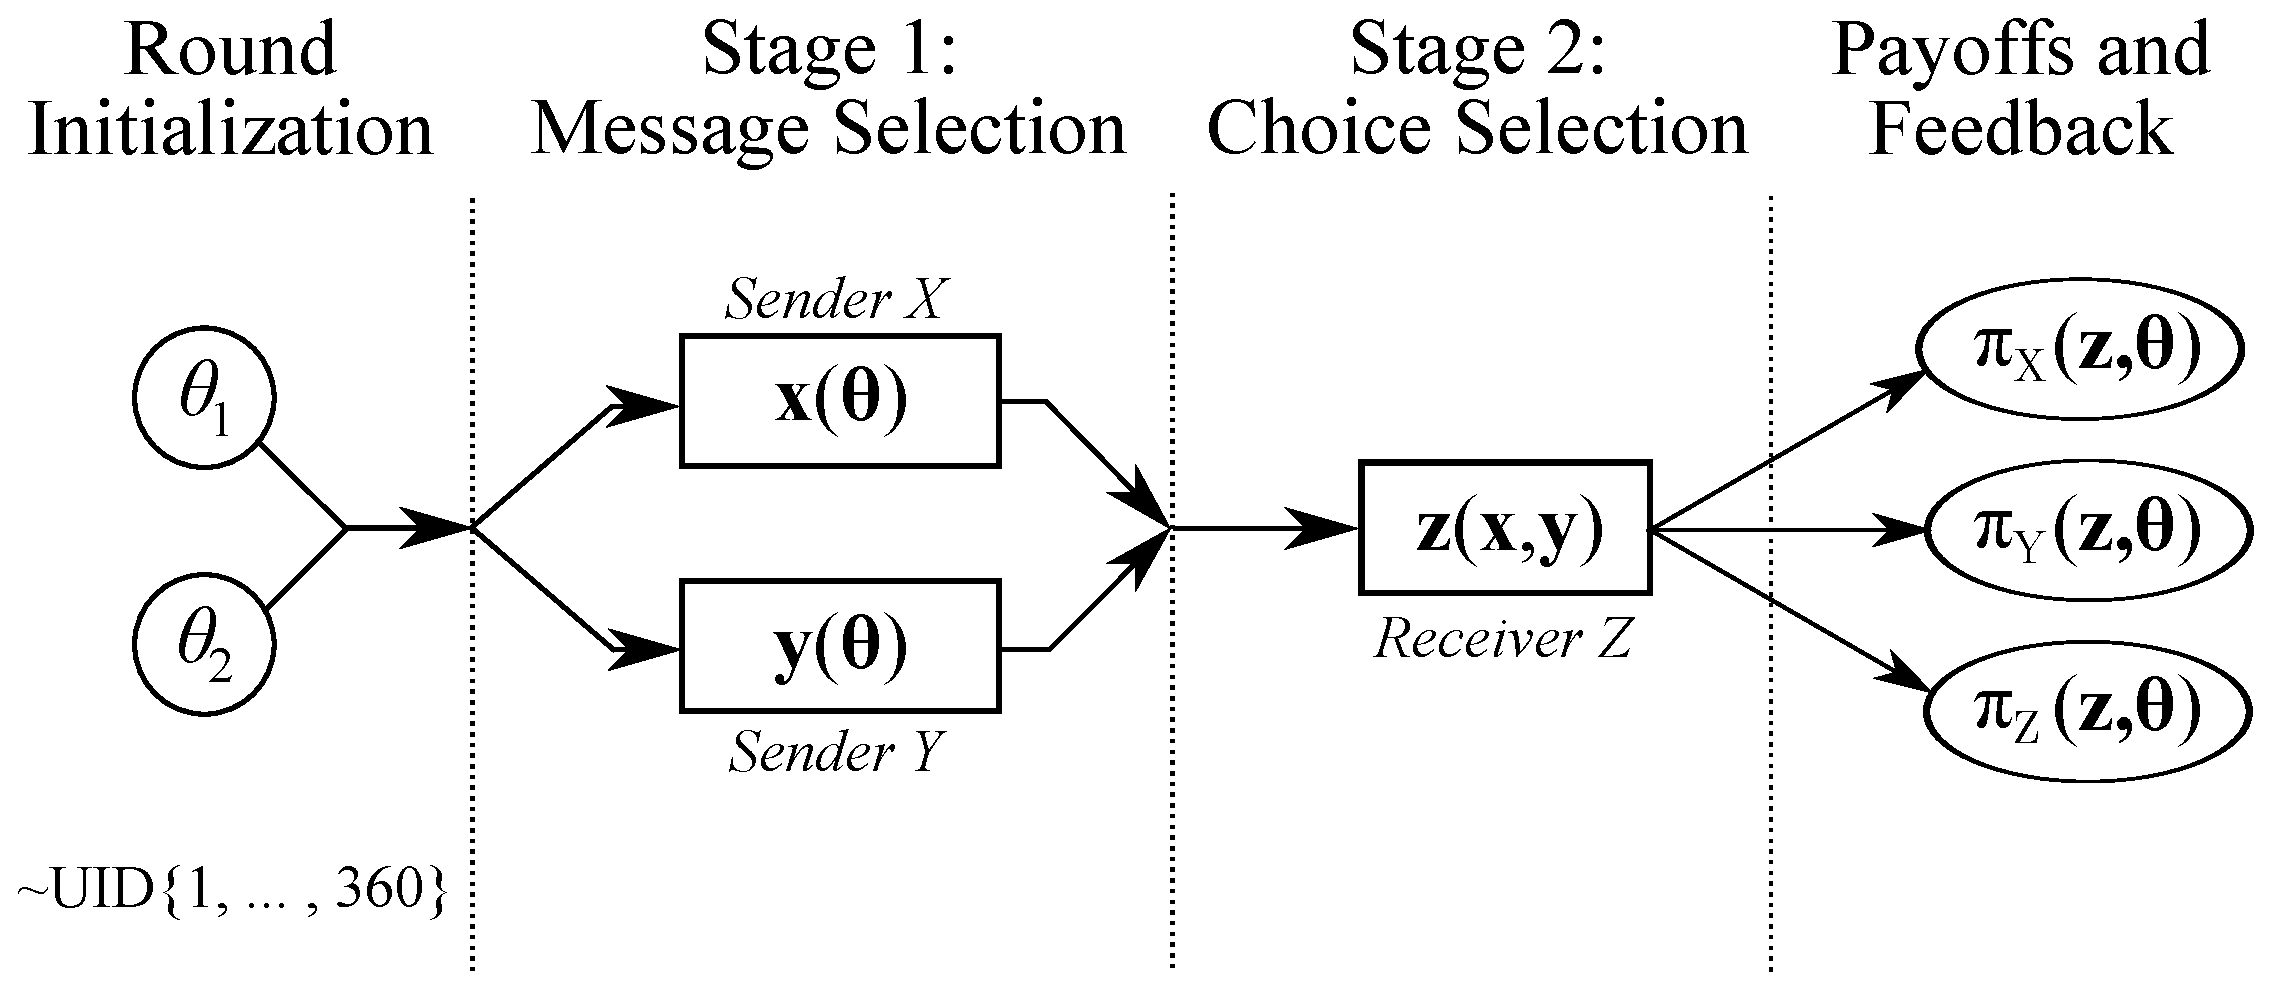
\includegraphics[width=0.8\textwidth]{../../../../ARCHIVE/vw_multi2/Images/Timeline.eps}

	\end{center}

\end{frame}


\subsection{Results}
\begin{frame}{}
Results...
\end{frame}
\begin{frame}{Message Exaggeration: Axis-Aligned}
	\includegraphics<1>[width=0.8\textwidth]{../../../../ARCHIVE/vw_multi2/Images/MessagesAAc_All.eps}
\end{frame}

\begin{frame}{Message Exaggeration: Symmetric Rotated}
	\includegraphics<1>[width=0.8\textwidth]{../../../../ARCHIVE/vw_multi2/Images/MessagesSRc_All.eps}
\end{frame}

\begin{frame}{Message Exaggeration: Asymmetric Rotated}
	\includegraphics<1>[width=0.8\textwidth]{../../../../ARCHIVE/vw_multi2/Images/MessagesARc_All.eps}

\end{frame}

\begin{frame}{Message Exaggeration: Perfectly Aligned Senders}
	\includegraphics<1>[width=0.8\textwidth]{../../../../ARCHIVE/vw_multi2/Images/MessagesUAc_All.eps}
\end{frame}

\begin{frame}{Message Exaggeration: One Sender}
	\includegraphics<1>[width=0.8\textwidth]{../../../../ARCHIVE/vw_multi2/Images/Messages1Sc_All.eps}
\end{frame}

\begin{frame}{Summary of message behavior}
	\begin{itemize}
		\item In both treatments senders provide messages close to the ray defined by their bias
		\item Slightly more exaggeration in the direction of opposition in the rotated environment
	\end{itemize}
\end{frame}

\begin{frame}{Extraction of Information, Payment CDFs}
	\begin{center}
	\includegraphics<1-3>[width=0.6\textwidth]{../../../../ARCHIVE/vw_multi2/Images/ChoiceDistanceCDF_FullToBabbling_circles.eps}
	\end{center}
	\only<1>{\color<1>{white}Median in axis aligned \$17.85}
	\only<2>{Median in axis aligned \$17.85}
	\only<3>{Median in symmetric rotated treatment,\$7.87}
\end{frame}
\begin{frame}{Extraction of Information, Counter-factual Payment CDFs}
	\begin{center}
	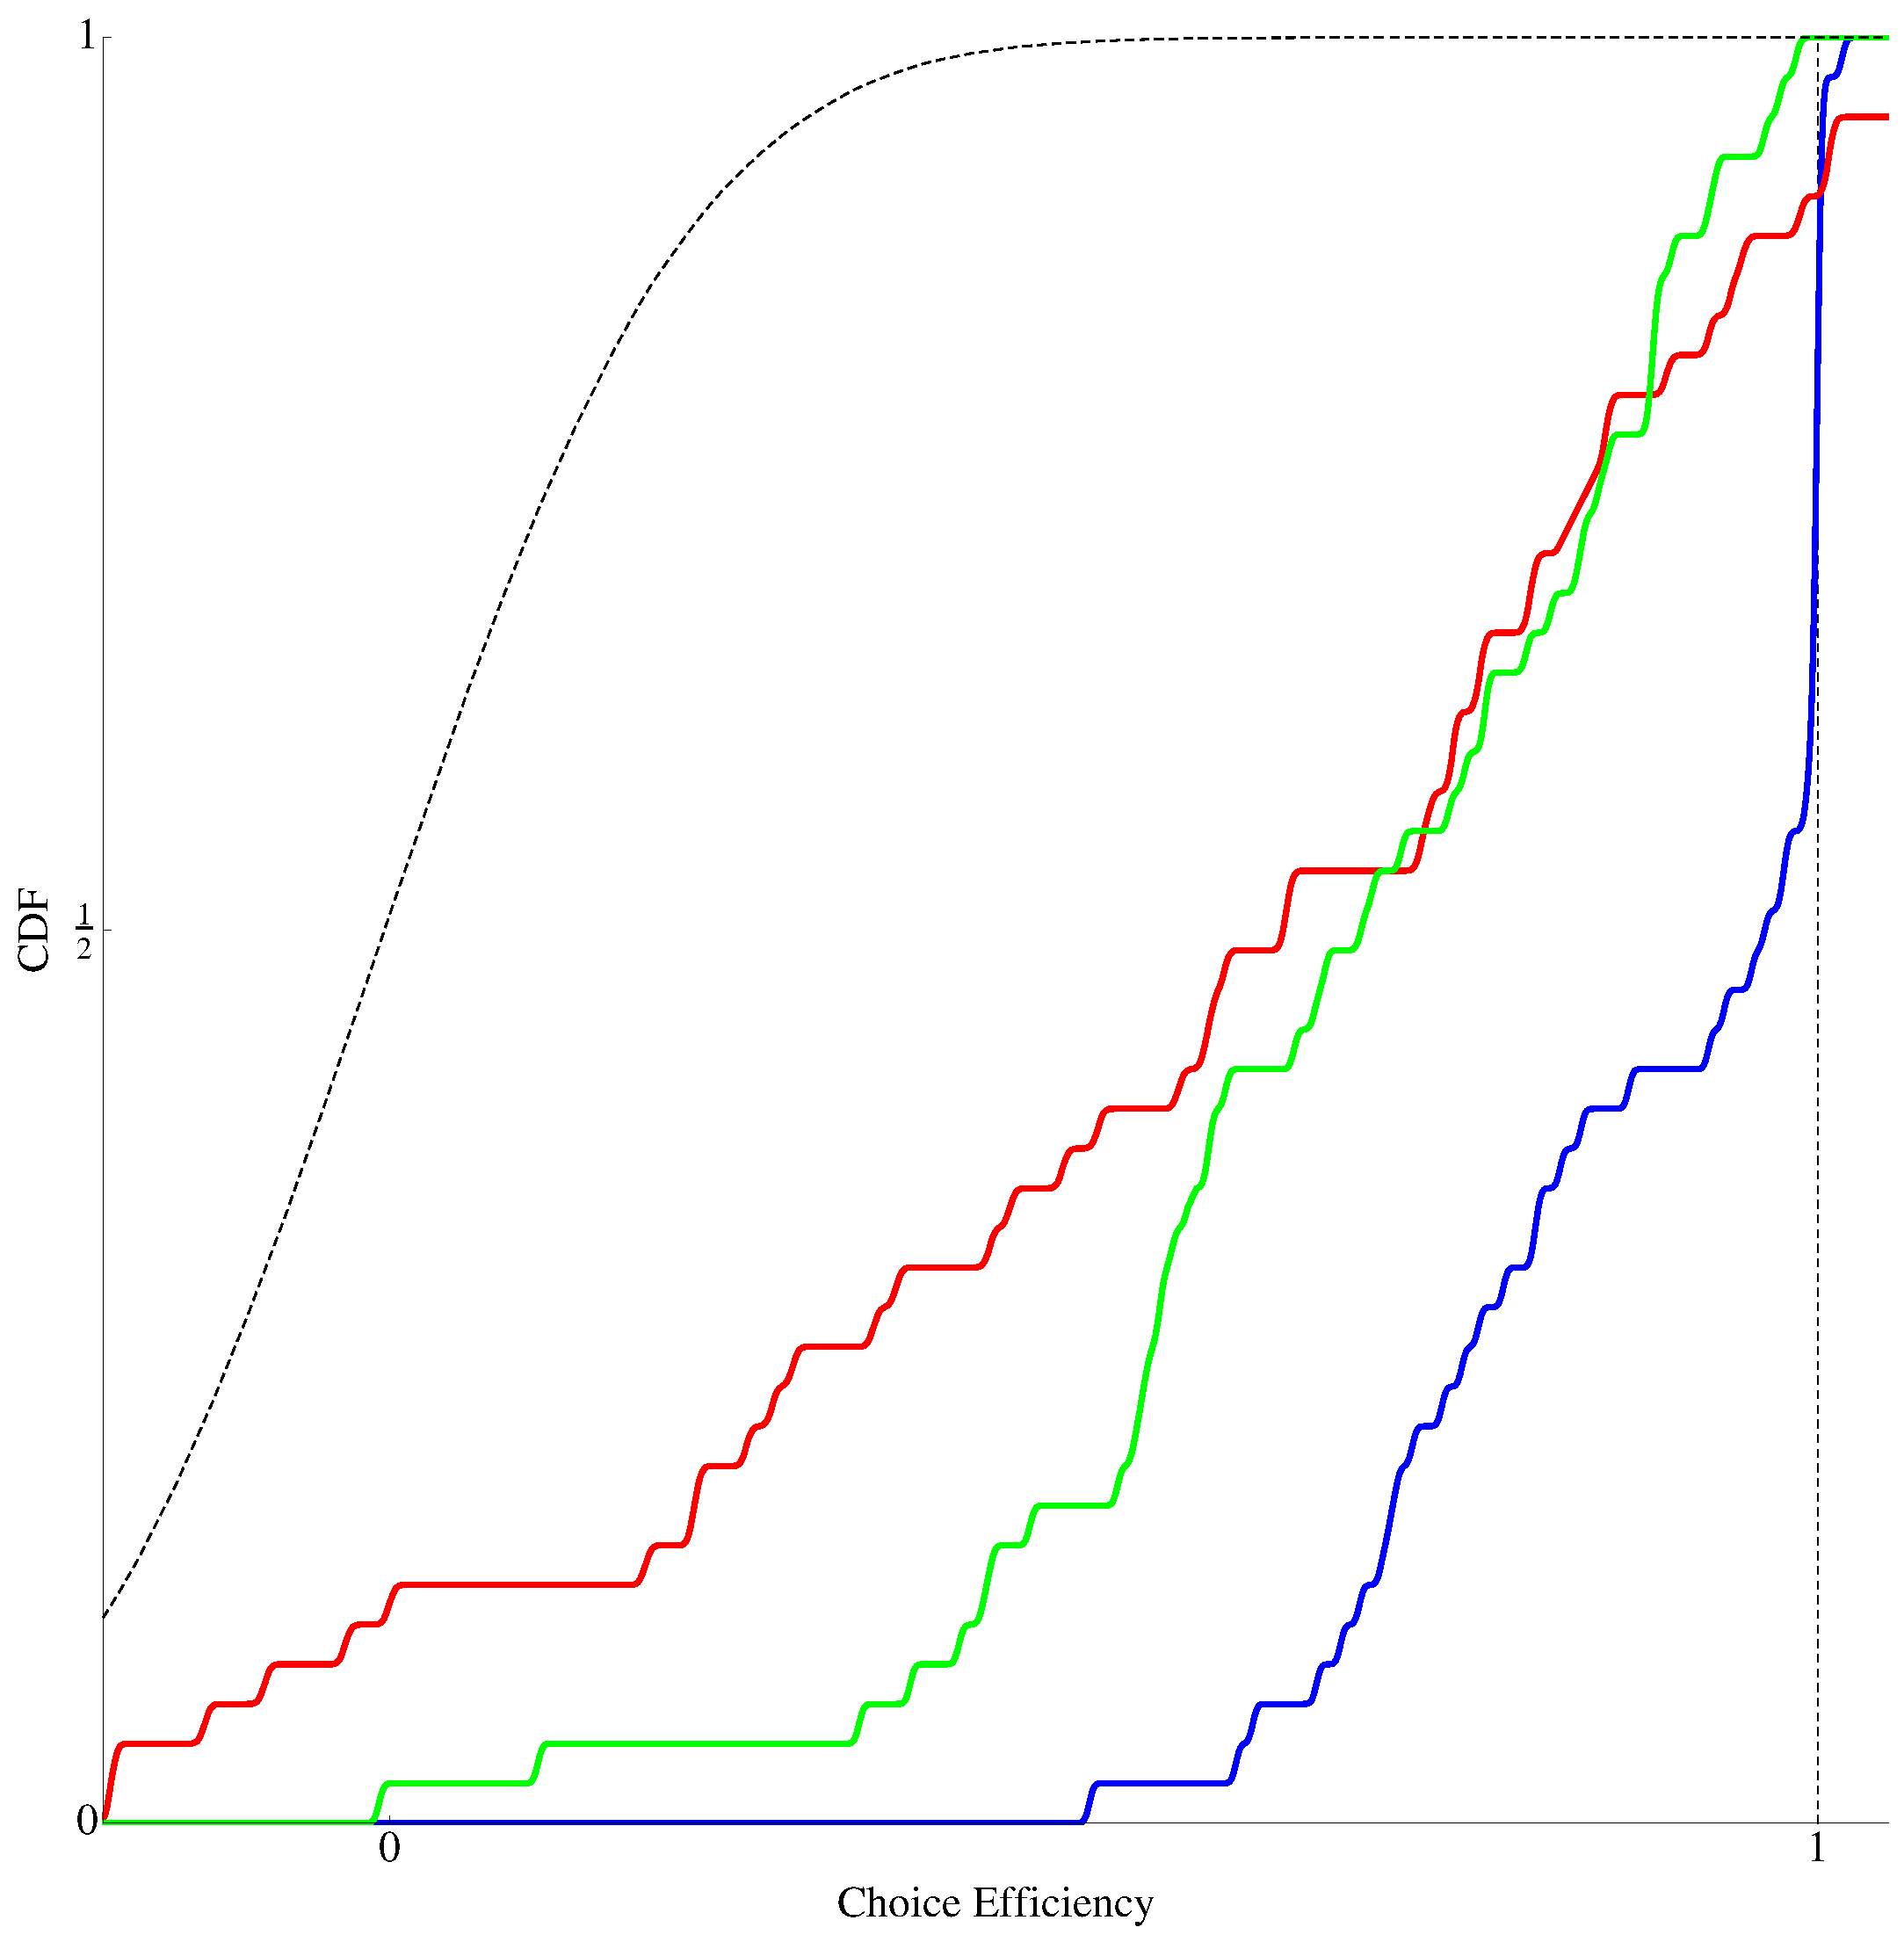
\includegraphics[width=0.6\textwidth]{../../../../ARCHIVE/vw_multi2/Images/BRChoiceDistanceCDF_FullToBabbling_circles.eps}
	\end{center}
	\only<1>{\color<1-2>{white} Text}
	\only<2>{Under equilibrium play, median in AA goes from \$17.85 to \$19.82}
	\only<3>{Under equilibrium play, median in SR goes from \$7.87 to \$13.83}
\end{frame}
\begin{frame}{Receiver strategies---Estimates}
	\begin{center}
		\begin{tabular}{lccccc}\hline
		 & \multicolumn{2}{c}{Theory} & & \multicolumn{2}{c}{Estimated}\\\cline{2-3}\cline{5-6}
		Treatment & $\alpha$ & $\beta$  & & $\hat{\alpha}$ & $\hat{\beta}$ \\ \hline
			AA  & 1.00 & 0.00 & &0.85 & -0.02 \\
			    & 0.00 & 0.00 & &0.15 & -0.08\\
			SR  & 0.50 & -0.50 & &0.42 &-0.09 \\
			    & 0.50 & 0.50 & &0.56 &-0.03 \\
			AR  & 0.74 & -0.44 & &0.67 &-0.05 \\
			    & 0.26 & 0.44 &  &0.38 &-0.05 \\ \hline
		\end{tabular}
	\end{center}
	\begin{itemize}
		\item Estimate the relationship:
			$$z^1_{it}=\alpha^1 x^1_{it}+(1-\alpha^1)y^1_{it} +\beta^1(x^2_{it}-y^2_{it}) +\epsilon^1_{it}$$
			$$z^2_{it}=\alpha^2 x^2_{it}+(1-\alpha^2)y^2_{it} +\beta^2(x^1_{it}-y^1_{it}) +\epsilon^2_{it}$$
	\end{itemize}
\end{frame}

% \begin{frame}{Receiver strategies}
	% \begin{itemize}
		% \item In the robust treatments we can can construct an axis system where one sender is completely aligned. $(x\mapsto \phi^s (x))$\pause
		% \item We can then ask, on this new axis, did the receiver trust the right sender \pause
		% \item Assess $\beta_i$ at subject-level, using the equations:
		% $$\boldsymbol{\phi}^s_{1}(\mathbf{z}_{it})=\beta_i\boldsymbol{\phi}^s_{1}(\mathbf{x}_{it})+(1-\beta_i)\boldsymbol{\phi}^s_{1}(\mathbf{y}_{it})+\epsilon_{i1t}$$
		% and
		% $$\boldsymbol{\phi}^s_{2}(\mathbf{z}_{it})=(1-\beta_i)\boldsymbol{\phi}^s_{2}(\mathbf{x}_{it})+\beta_i\boldsymbol{\phi}^s_{2}(\mathbf{y}_{it})+\epsilon_{i2t}$$
	% \end{itemize}
% \end{frame}
% \begin{frame}{Which Sender do Receivers Trust? (Pooling)}
	% \includegraphics[width=0.8\textwidth]{../../../../ARCHIVE/vw_multi2/Images/ReceiverTrustCDF.eps}

	% \showOn{Almost half the subjects in the Axis Aligned treatment use an equilibrium rule.}{2-3}{1}

	% \showOn{But no-one in the rotated treatments comes close}{3}{1-2}
% \end{frame}


% \begin{frame}{Which Sender do Receivers Trust? Aligned}
	% \includegraphics[width=0.8\textwidth]{../../../../ARCHIVE/vw_multi2/Images/ReceiverEqbmRulesAA.eps}
% \end{frame}

% \begin{frame}{Which Sender do Receivers Trust? Rotated}
	% \includegraphics[width=0.8\textwidth]{../../../../ARCHIVE/vw_multi2/Images/ReceiverEqbmRulesSR.eps}
% \end{frame}

\begin{frame}{Receiver strategies}
	\begin{itemize}
		\item Look at the dimension $i$ on which the subjects are opposed.
		\item The recommendations $x_i$ and $y_i$ should lie either side of the true state\pause
		\item Whereabouts do senders locate on the interval between these two messages:
		$$\alpha_i=\frac{z_i-x_i}{y_i-x_i} $$\pause
		\item If the biases are symmetrically opposed, locate toward the sender you trust more
	\end{itemize}
\end{frame}

\begin{frame}{Location of decision between opposed senders}
	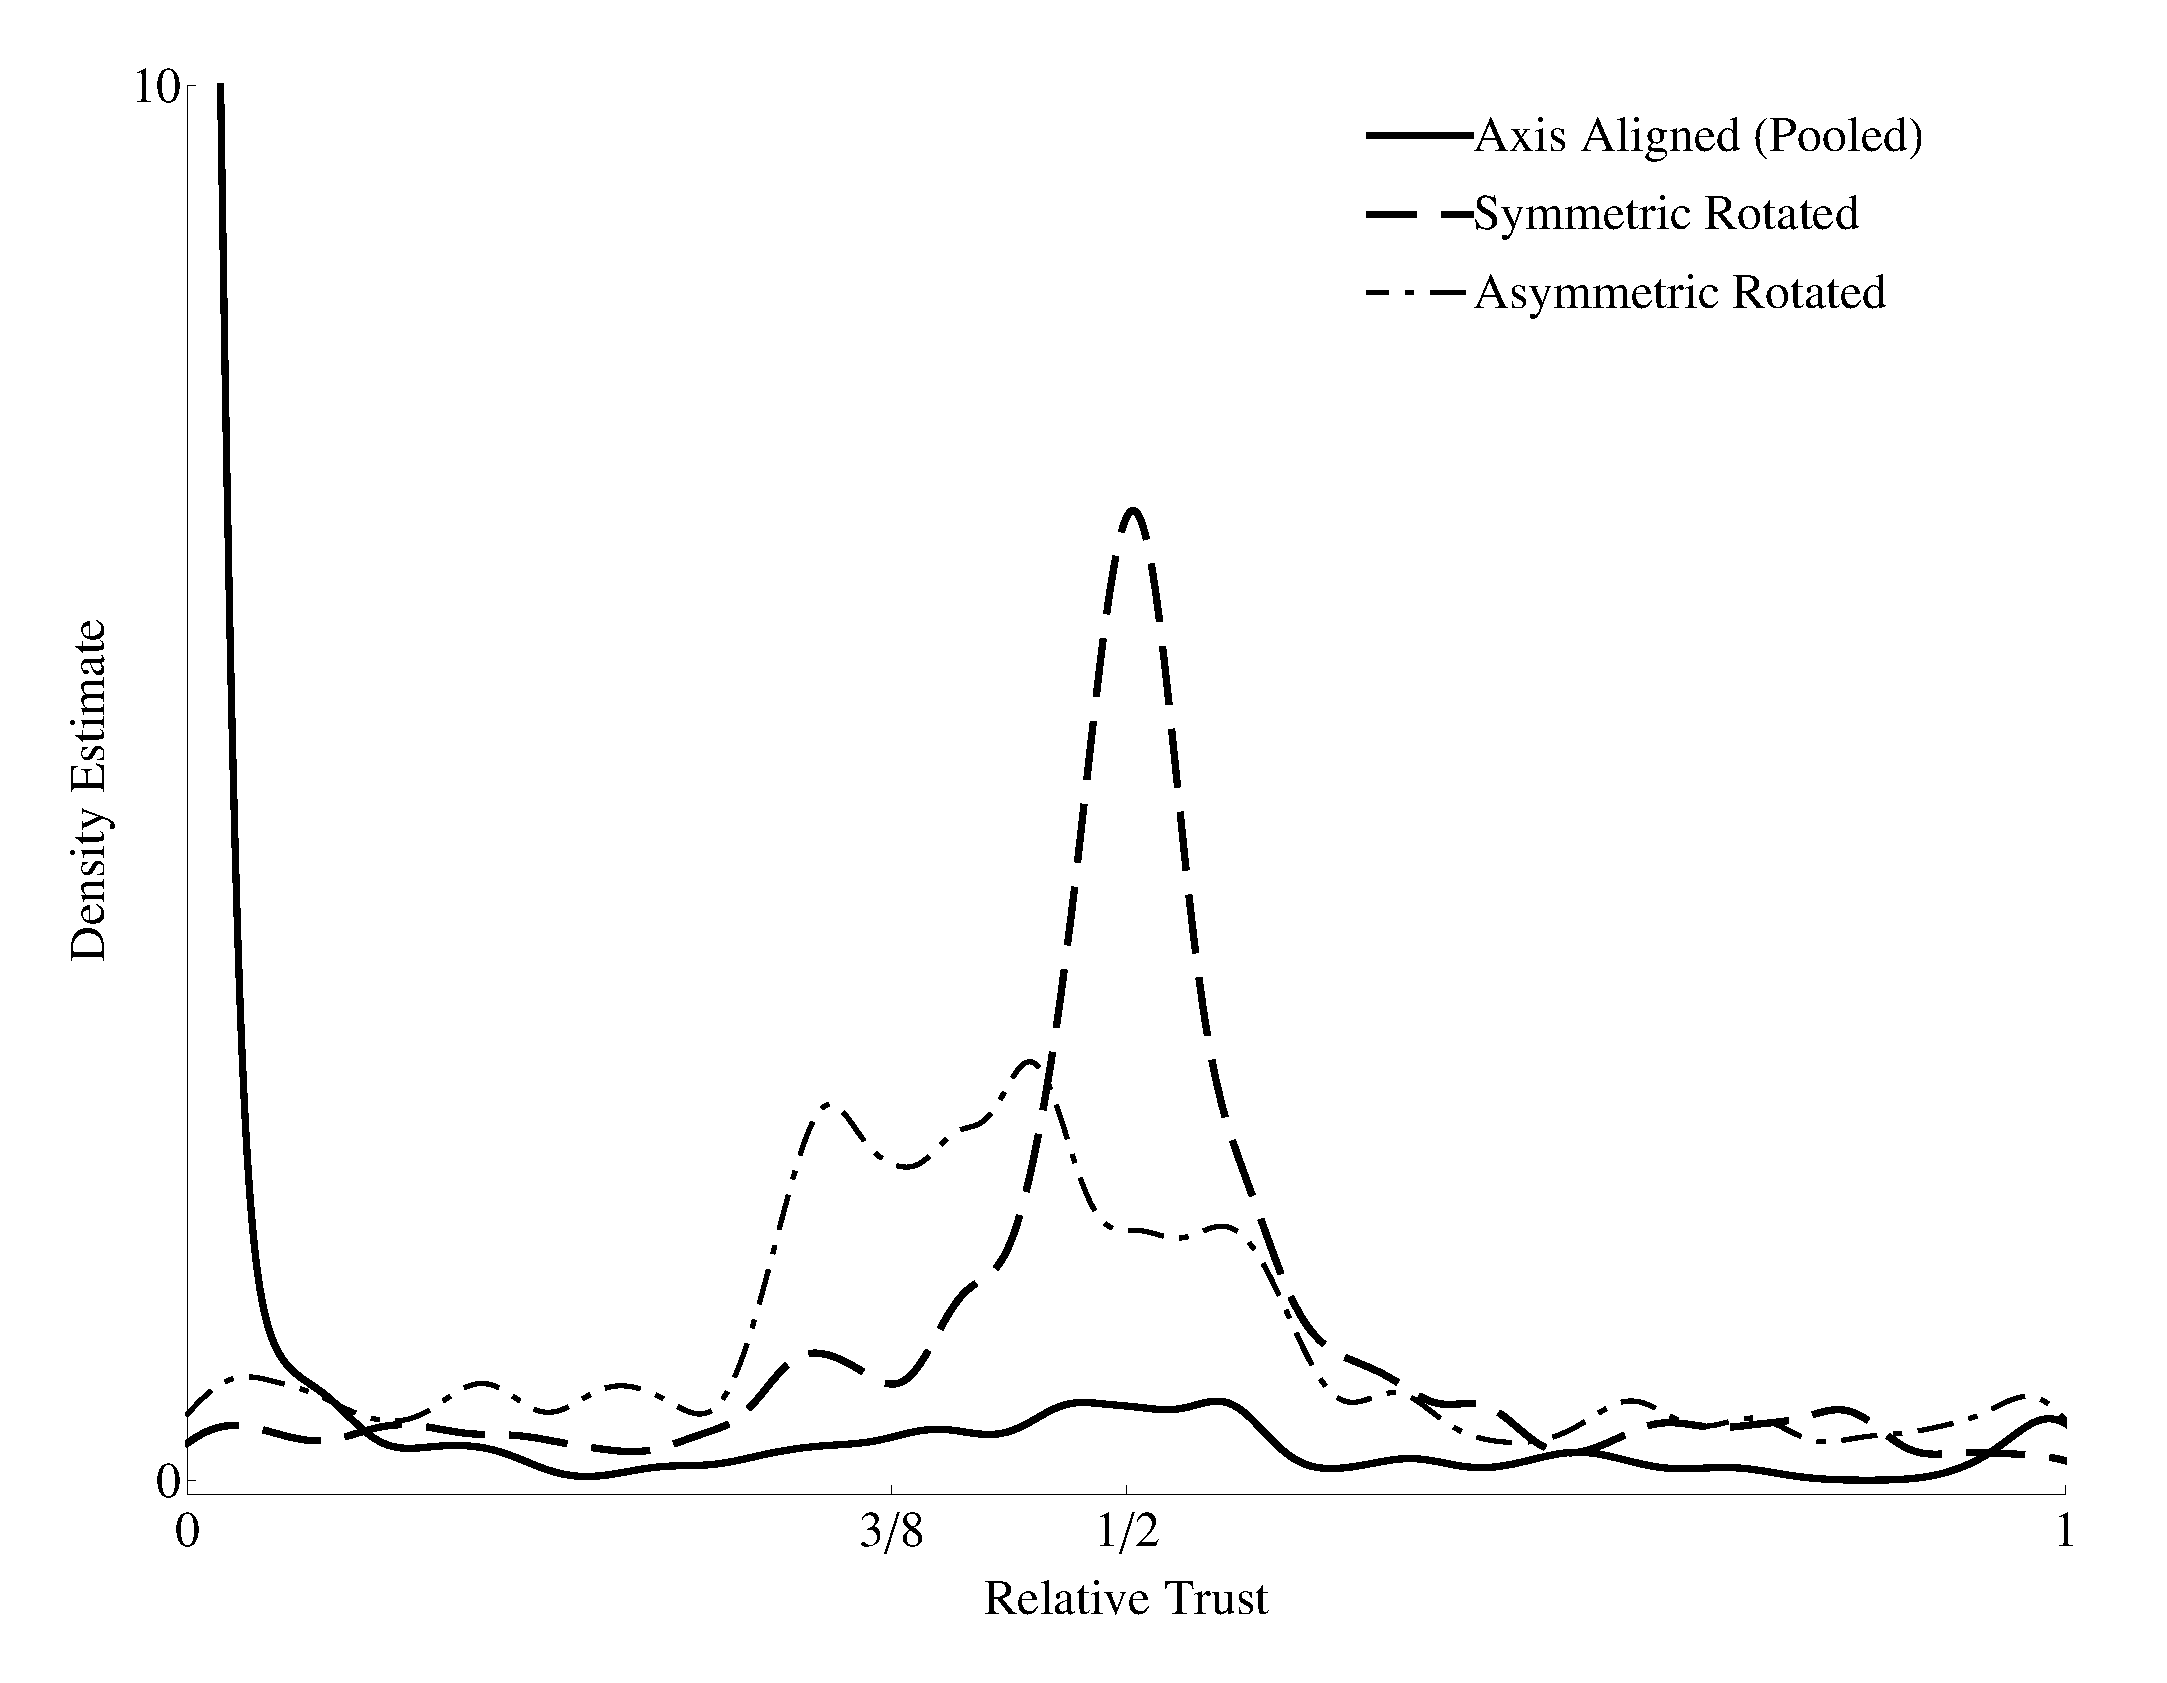
\includegraphics[width=0.8\textwidth]{../../../../ARCHIVE/vw_multi2/Images/OpposedSenderTrust_KernelM.eps}
\end{frame}

\begin{frame}{Unidimensional Response---Axis Aligned}
	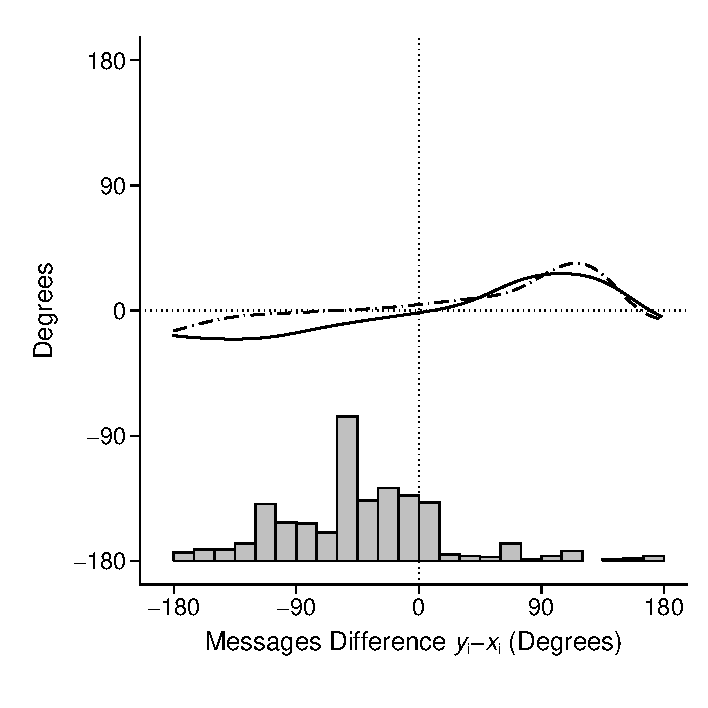
\includegraphics[width=0.8\textwidth]{../../../../ARCHIVE/vw_multi2/Images/ConditionalChoiceWHist_AA_2.eps}
\end{frame}

\begin{frame}{Unidimensional Response---Symmetric Rotated (Opposed)}
	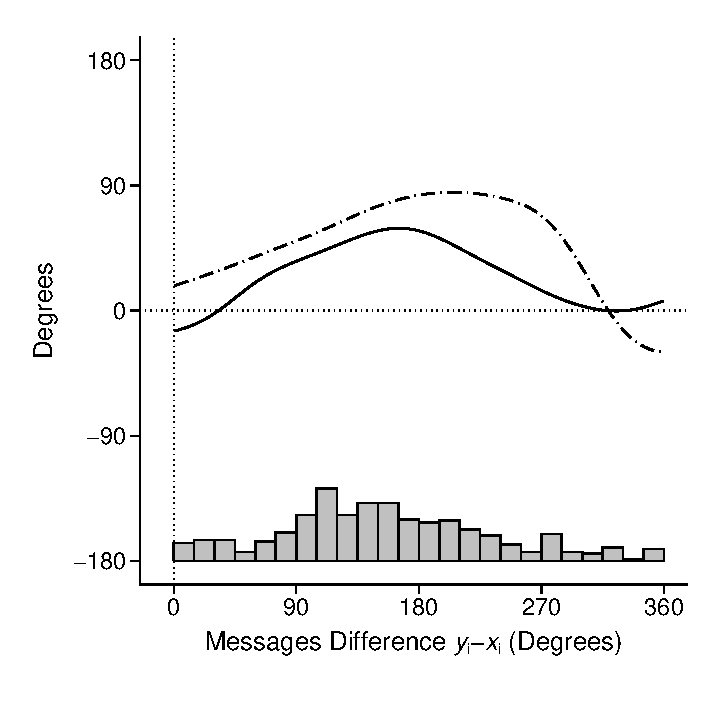
\includegraphics[width=0.8\textwidth]{../../../../ARCHIVE/vw_multi2/Images/ConditionalChoiceWHist_SR_1.eps}
\end{frame}
\begin{frame}{Unidimensional Response---Symmetric Rotated (Aligned)}
	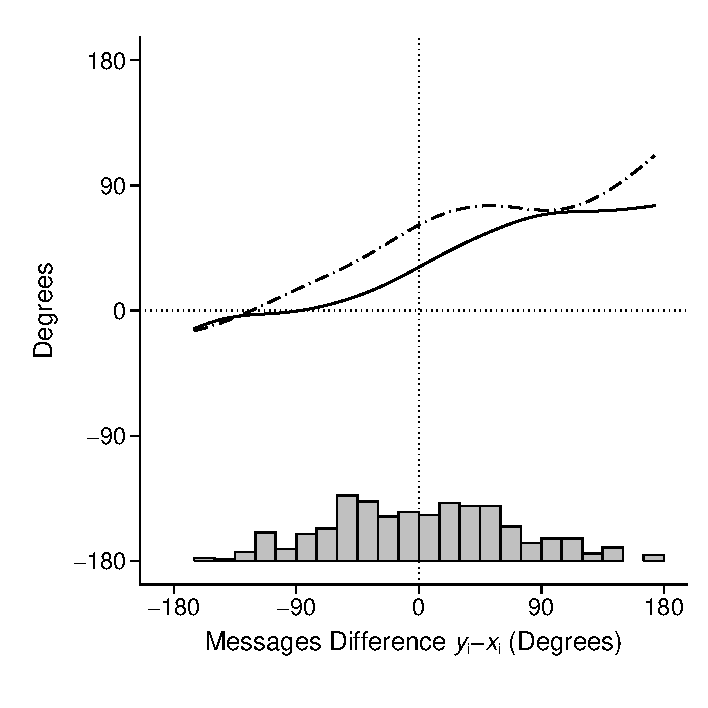
\includegraphics[width=0.8\textwidth]{../../../../ARCHIVE/vw_multi2/Images/ConditionalChoiceWHist_SR_2.eps}
\end{frame}

\begin{frame}{Location of decision between opposed senders}
	\begin{itemize}
		\item But in the rotated treatments the equilibrium requires receivers to react more to the recommendations of those who seem trustworthy in the other dimension
		\item We regress the point in between the opposed signals $\alpha_it$ on which sender seemed more trustworthy
		\item Find no significant effects \pause
		\item {\bf Conclusion: receivers only react to \emph{ex ante} trustworthiness, not to the information contained in the signals}
	\end{itemize}
\end{frame}

\begin{frame}{Summary}
	\begin{itemize}
		\item Simple graphical implementation of Battaglini (2002)
		\item Very little \emph{Honest} revelation by senders
		\item Subjects are much more successful at extracting information in the Axis-Aligned environment
		\item Once biases become more complex receivers do not extract information optimally, despite large potential gains
		\item Subjects only react to \emph{ex ante} trust in senders
	\end{itemize}
\end{frame}

% \begin{frame}
% \begin{center}
% \framebox{\includegraphics[height=0.75\textheight]{../../../../Deliberation/Images/G.eps}}
% \end{center}
% \end{frame}
\end{document}


